\section{Evaluation and Model}

% show measurement results and explain that headers are parsed for xconnect/bridging even if they are not needed \ref{}

% mention the missing mac addr setting in vpp16.09

% talk about max fib sizes

% mention that for fibs only one via target is used as in rfc defined

% how well does the fantastic memory alignment of vpp work in numa?


\subsection{CPU as the Bottleneck}
\label{sec:cpubottleneck}

Table \ref{table:bottleneck} presents maximum throughput of all
measured scenarios with minimum sized packets using a single \Ac{vpp}
worker. 

The results show, that the computationally least expensive scenario (xconnect) allowes for the highest packet rates. 

\begin{figure}[!ht]
	\vspace{5ex}
	\begin{tabular}[]{ l r r r }
		Scenario & 1.2GHz (50\%) & 3.1GHz (97\%)  & 3.2GHz (100\%) \\ 
		\midrule
		xconnect & 7.34 (56\%) & 12.90 (98\%) & 13.20 (100\%) \\ % stdDev 0.03 0.02 0.12
		l2 bridge no features & 6.69 (55\%) & 11.84 (97\%) & 12.18 (100\%) \\ % 0.01 0.03 0.08
		l2 bridge mac-learn, mac-age & 6.05 (55\%) & 10.84 (98\%) & 11.09 (100\%) \\ % 0.01 0.05 0.02
		IPv4 1 route & 6.03 (53\%) & 10.98 (97\%) & 11.28 (100\%) \\ % stdDev 0.01 0.02 0.05
		IPv4 255k routes & \\
		IPv6 1 route & \\
		IPv6 255k routes & \\
		VXLAN encap & \\
		\midrule
	\end{tabular}
	\caption{Maximum througput (Mpps) in different scenarios with different CPU frequencies measured on klaipeda. }
	\label{table:bottleneck}
\end{figure}
% With offered Mpps beeing 100\%, "Relative" is the maximum packet throughput in relation to the offered one.


\subsection{Throughput and CPU Scaling (Model)}

Since the CPU is a bottleneck in all tested configurations, the
ability to distribute the load over multiple CPU cores is
essential. Not all \Ac{vpp} configurations support this though.

\Ac{vpp} has two concepts for using multiple cores: It has workers for
simultanous recieving and processing of packets over the processing
graph - and it can be configured to use another set of workers for
proiritized sending of packets (\Ac{hqos} \cite{vppdocs:qos}
\cite{vppdocs:hqosplacement}). Only the first type of worker can be
used to enhance the performance of raw processing throughput though.

Many layer 3 processing nodes such as the \Ac{ip4} and the \Ac{ip6}
processing path do support parallel packet processing using \Ac{rss}
(see section \ref{sec:rss}). For the scaling to have effect, the
packets need different packet headers though, so that \Ac{rss} header
field hashing can assign them to different queues.

% TODO what happens with different flows per core? low flows but high core count?

% simple cpu scaling on klaipeda 10GbE and omanyte 40GbE
% maybe show both with high and low cpufreq
% klaipeda easily saturated with 2 links
% omanyte with lower freq shows good scaling up to 4 cores

% singlethreaded is typically a ~x% slower than main thread and a single worker


% \begin{figure}[!ht]
% \noindent\hspace{0.5mm}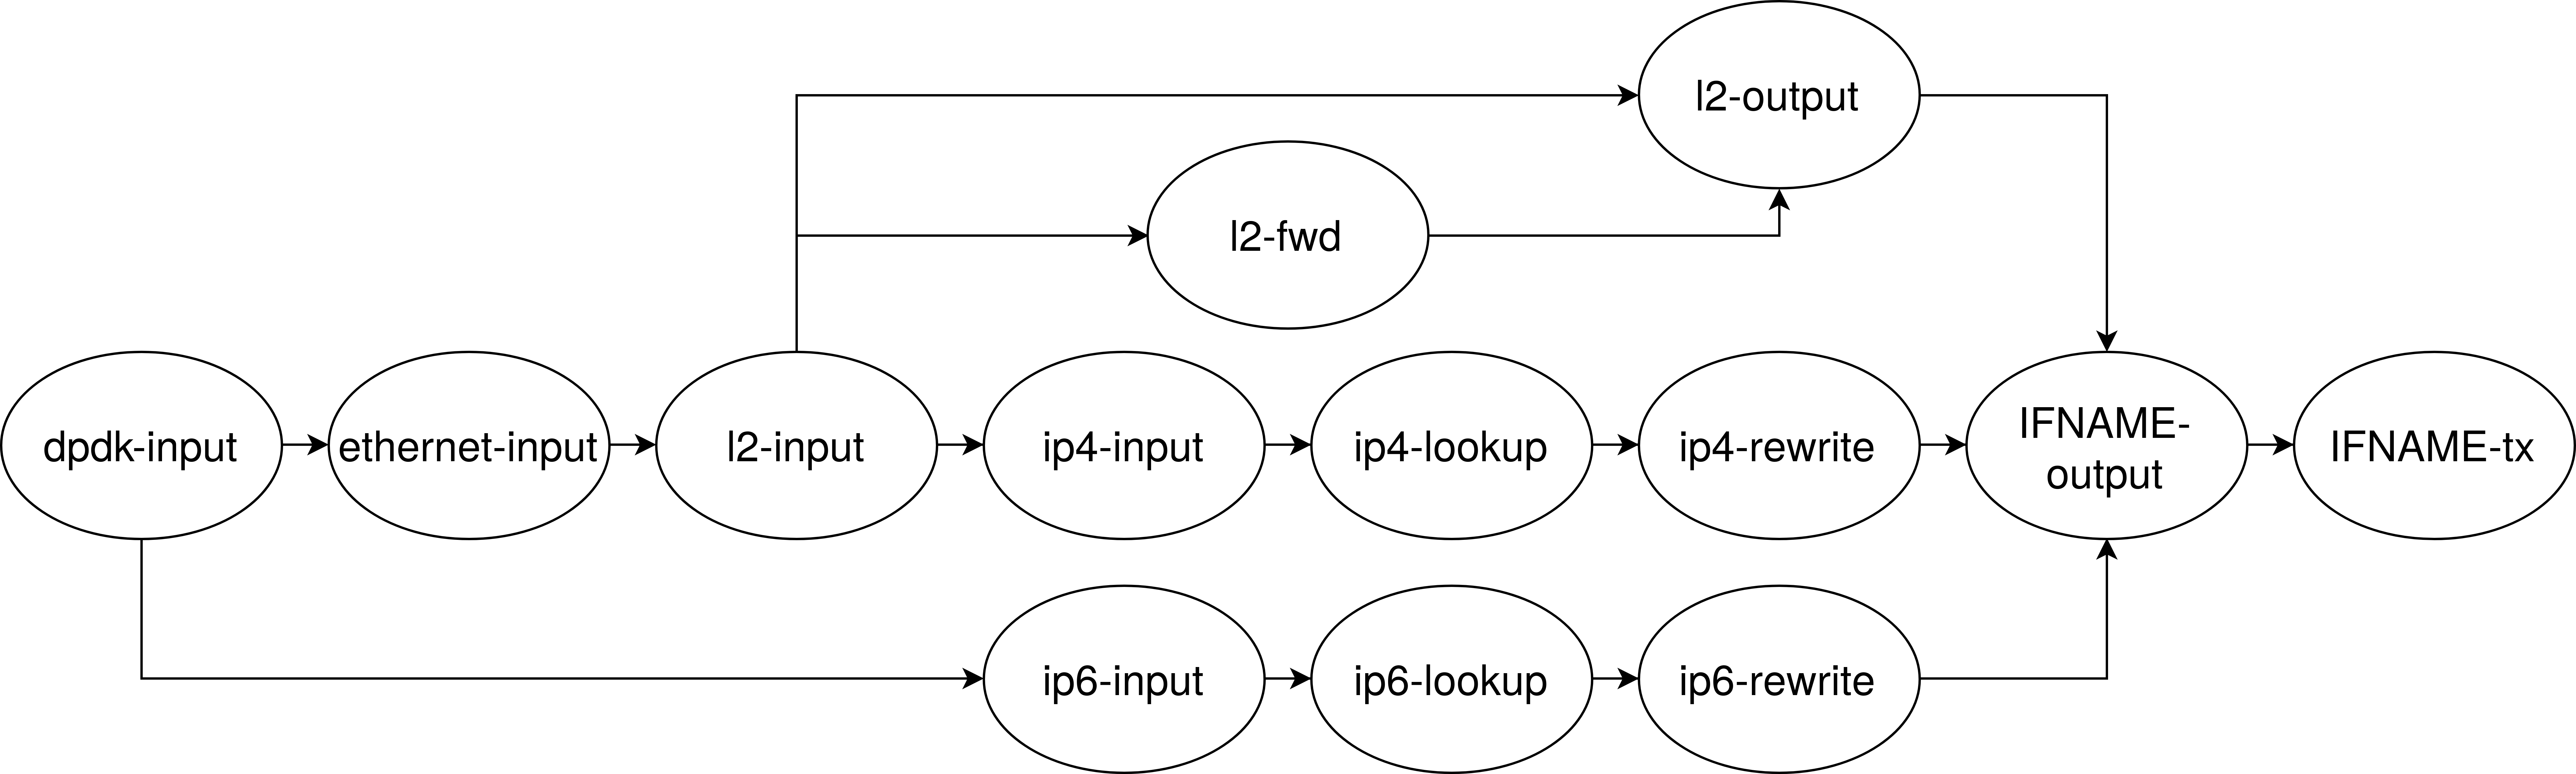
\includegraphics[width=\linewidth]{pics/vpp-nodes-horizontal.png}
% \caption{VPP packet processing graph for xconnect, bridging, ip4 routing and ip6 routing. Other paths are left out. }
% \label{nodegraph}
% \end{figure}


\subsection{Forwarding Tables (Model)}

$2^{24}$

% TODO fix nachkommastellen

\begin{figure}[!ht]
	\vspace{5ex}
	\begin{tabular}[]{ l r r r }
		Implementation & FIB size & Mpps & Relative \\ 
		\midrule
		MoonRoute & 1 & 14.6 & 100\% \\
		MoonRoute & $2^{20}$ & 14.2 & 97\% \\
		MoonRoute & $2^{24}$ & 11.6 & 79\% \\
		VPP v18.10 & 1 & 11.56 & 79\% \\
		FastClick DPDK & 1 & 10.4 & 72\% \\
		FastClick DPDK & $2^{20}$ & 10.4 & 72\% \\
		VPP v16.09 & 1 & 9.69 & \\
		VPP v16.09 & 255k & 9.20 & \\
		VPP v16.09 & $2^{20}$ & 8.50 & \\
		VPP v18.10 & 255k & 7.23 & 50\% \\
		VPP v16.09 & $2^{23}$ & 6.53 & \\
		Click DPDK & 1 & 4.3 & 29\% \\
		Click DPDK & $2^{20}$ & 4.2 & 28\% \\
		Linux 3.7 & 1 & 1.5 & 11\% \\

		\midrule
	\end{tabular}
	\caption{Comparison of maximum \Ac{ip4} forwarding throughput with a single worker on klaipeda (see table \ref{table:hardware}). Non-VPP results are from \cite{chair:architecture}}
	\label{table:comparison}
\end{figure}

% present measurement results_
% - l2fib
% - v18.10
% 	- ip4
% 	- ip6
% - v16.09

% model the performance decrease according to causes

% cpu scaling and live inserts

\subsection{Latencies (Model)}




\subsection{Bottleneck Analysis}

- fib: memory cache speed
- cpu cycles
- other hardware bottleneck? but this was already written about in analysis

\subsection{performance decrease over versions}